\section{Background}

In April 2019, LSST DM began a proof of concept project with the AWS and HTCondor teams to explore whether a cloud deployment of the Data Release Production (DRP) is feasible.
The execution plan of the project is described in DMTN-114.
For this project AWS granted us credits to use their platform.
The team met biweekly to discuss the progress and plans.
In this document we report the results.


\section{Approaches and Strategies}

In executing this PoC we focused on the goal of being able to demonstrate the data processing on the AWS cloud and kept the following strategies in mind.

\begin{enumerate}
\item
Progress in phases.
Following the ideas in DMTN-114 we started with simply moving the execution to a cloud instance without modifying any backend, and gradually switching out each component to use AWS products.
Amazon's Network File System, Amazon Elastic File System (Amazon EFS), was used in the first phase as the storage of a shared data repository, before the S3 datastore could be used directly via the Data Butler interface.
A sqlite file on Amazon EFS was as the Data Butler Registry before we moved it to an Amazon RDS instance.
A Personal Condor Pool on one instance was used before we tested the capability to launch new instances as the Condor workers.
This approach allowed us to debug and adapt more smoothly and always had a fallback option in integrating and testing new features and components.
\item
Test with small tasks and dataset before scaling up.
In particular, the \texttt{ci\_hsc} \href{https://github.com/lsst/ci\_hsc} dataset and the CI workflow provide a minimal HSC test dataset and a representative DRP workflow and algorithms.
The test workflow was always run as one of the first integration steps.
\item
Use Gen3 middleware.
One of the mandates in the PoC was to use the Gen3 Middleware, which is designed to ease the DRP execution and automation compared to the previous Gen2 Middleware.
However, as the Gen3 Middleware has been under active development during the course of the PoC, there were many backwards incompatible changes, the API and registry schema were unstable, no Gen3 continuous integration tests existed when we first started, and the test coverage was not good.
We did not always follow the bleeding edge version and updated only when unnecessary, such as important bug fixes.
Nonetheless the stack versions should not have strong impacts in the PoC conclusions.
\item
Focus on end-to-end execution and leave optimization behind.
Some potential optimizations and further investigations were identified throughout the PoC project but were not carried out.
Ideas are described in Sec \ref{future}.
\end{enumerate}


\section{Architecture Design}

The system design in the end of the PoC is as in the diagram in Figure~\ref{fig:arch}.
All components are hosted on the AWS platform.

\begin{figure}
  \centering
  \includegraphics[width=\textwidth]{figures/arch}
  \label{fig:arch}
  \caption{architecture design}
\end{figure}

The user launches an on-demand instance as the master submit host and the central manager of the HTCondor.
HTCondor manages an HTCondor pool which is a collection of resources.
On the master, the command line interface of Pegasus is used to submit, control, and monitor the LSST workflow.
Each LSST Pipeline Task quantum is mapped into a Pegasus job in the abstract workflow which is resource-independent.
The job dependency is represented as a directed acyclic graph (DAG).
Pegasus adds other necessary jobs, such as data transfer, to the executable workflow.
HTCondor DAGMan is the workflow execution engine behind Pegasus and controls the processes.
HTCondor match jobs with available resources.

Using HTCondor Annex, AWS EC2 instances are launched as workers to join the HTCondor Pool.
Either the on-demand or the Spot instances can be added.
Fleets of multiple Spot instances can be requested using HTCondor Annex commands.
HTCondor Annex manages the instance lifecycle.

LSST Pipeline jobs are executed on the worker instances.
Science files are stored in a S3 bucket which is a Data Butler Datastore, and pipelines jobs read and write directly to the S3 bucket.
Pipeline jobs also connect directly to the RDS instance which is the Data Butler Registry that keeps track of the science files.
These new Data Butler backends were implemented during the PoC, see Sect \ref{butler}.

Files that are not managed by Data Butler are managed by the Condor File IO via Pegasus.
These include the Data Butler configuration file, pipeline definition (Quantum Graph) files, and the log files.
The master instance also serves as the staging site for these files.
Condor File IO transfers input and output files between the master and the workers; instances do not share a filesystem.


\subsection{Alternative architecture designs were also discussed in the PoC}

We discussed different architecture designs but did not pursue all of them due to time constraints.
One prominent idea is to use condor transfer to read and write files to S3, rather than relying on Data Butler to communicate directly with S3.
A new plug-in to do so has been recently added in HTCondor.
In this design HTCondor controls all file transfer.

Similarly, database ingestion may be done only after the jobs fully finish, rather than one at a time while the jobs run.
This also may reduce the number of database connections by bundling transactions from multiple jobs together.
The idea here is to handle database transactions in a centralized manner, not on workers, so can have a limited number of database connections.
This design may require a local sqlite registry to be used in each job.
Job wrappers and new Data Butler features may be needed.


\section{Building AWS support into the Data Butler and lessons learned}

The Data Butler is the overarching data IO abstraction through which all LSST data access is mediated. Datasets are referred to by their unique IDs, or a set of identifying references, which are then resolved through an registry that matches the dataset IDs, or references, to the location, file format and the Python object type of the dataset. The system that persists, reads and potentially modifies the datasets is called the datastore. The Registry almost always backed by an SQL database and the Datastore is usually backed by a shared filesystem. A major focus of AWS POC was to implement, and investigate issues related to, an S3 backed Datastore and a PostgreSQL backed Registry.

Simple Storage Service (S3) is object storage provided by AWS. Unlike the more traditional file systems that manage data as a file hierarchy, or data blocks within sectors and tracts, objet storage manages data as objects. This allows the storage of massive amounts of unstructured data where each object typically includes the data, related metadata and is identified by a globally unique identifier. S3, specifically, promises 99.999999999\% durability as uploading an object to it automatically stores it across multiple systems, thus also ensuring scalability and performance. Related objects are generally stored in the same Buckets for easier administrative purposes. Access, read, write, delete and other atomical units of action on the objects themselves can be allowed or forbidden at the account, bucket or individual object level. Logging is available for all actions on the Bucket level and/or at the individual object granularity. It is also possible to define and issue complex alert conditions on Bucket or object actions which can execute arbitrary actions or workflows.

PostgreSQL is one of the most popular open source relational database systems available. The choice to go with PostgreSQL was based on the fact that it's a very popular and well supported open source software that suffers from no additional licensing fees usually associated with proprietary software. Relational Database Service (RDS) is the AWS cloud service that launches and configures databases with ease. 

At the time the AWS POC Group began generation 3 Butler, the latest implementation of the Data Butler, implemented PosixDatastore, a local or shared filesystem datastore, and a SqliteRegistry. OracleRegistry followed soon after LSST AWS POC group began work. Initialy the focus was on implementing an S3 backed datastore called S3Datastore. The interface between AWS services and LSST Stack would be based on the official AWS SDK called boto3. In March 2019, Dino Bektesevic visited NOAO to work more closely with Tim Jenness, which prooved to be instrumental in implementing the early versions of a new module in the `daf\_butler` called `s3utils`, an `S3Datastore` class, the PosixDatastore equivalent, and a set of appropriate unit tests that demonstrated its functionality and correctness. The unit tests for the datastore utilize the `moto` library which mocks requests and responses sent to AWS services, so that no additional external infrastructure is required to use it. PostgreSqlRegistry class was implemented partially during the visit and completed shortly after the visit. The initial implementation showcasing the required changes to the code was submitted as a Draft Pull Request \href{https://github.com/lsst/daf_butler/pull/147}{PR-147}. 

The tentative implementation revealed issues with how the Data Butler treated Uniform Resource Identifiers, or URIs, which were, at the time, not being handled correctly, as per standards defined in \href{https://tools.ietf.org/html/rfc3986}{FC-3986}, by The Location class. After expansive discussions and an example re-implementation called S3Location to demonstrate the issues, in May 2019 Tim Jenness authored the `ButlerURI` class (\href{https://github.com/lsst/daf_butler/pull/167}{PR-167}) resolving the issues. Major efforts were then invested into refining the newly added code to the level of production quality as well as updating the remaining Gen. 3 Butler to use the updated ButlerURI code instead. Every call to OS functionality had to be generalized to take a URI and from it determine the appropriate operation - a call to OS functionality, a AWS operation or something else. This led changes in Butler, Config, ButlerConfig and YAML Loader classes. These changes made the whole of Data Butler more general and pliable to future changes, such as adding support for other cloud providers. 

Further integration of the S3 backend required a change to Formatter classes to enable data serialization and deserialization to and from bytes. Formatters present interfaces for reading and writing of Python objects to and from files. They are the mechanism underlying how Data Butler is capable of presenting data as science products in the form of Python objects, abstracting away the underlying file types. Modifications were made to JsonFormatter, PickeFormatter, YamlFormatter, PexConfigFormatter and the generic abstract class Formatter. This concluded the last of changes required for S3Datastore integration. After which Jenkins integration tests were run and the S3Datastore and supplemental code was merged to master branch of the `daf\_butler` repository in \href{https://github.com/lsst/daf_butler/pull/179}{PR-179} (the associated Jira ticket is \href{https://jira.lsstcorp.org/browse/DM-13361}{DM-13361}). It became apparent that there are certain similarities that are shared between PosixDatastore and S3Datastore, similarities that would be shared by other future datastore implentations. To reduce code duplication the general datastore code was refactored and reorganized in \href{https://github.com/lsst/daf_butler/pull/187}{PR-187} shortly after. 

PostgreSqlRegistry was not part of this PR. The initial implementation was based on OracleRegistry, due to the similarities between the two, but was re-implemented in terms of the generic SqlRegistry class in July. Problems were caused, for both Oracle and PostgreSQL, by the table naming conventions and additionally, for PostgreSQL, the table views did not conform to the assumptions made. In July the PostgreSqlRegistry was re-implemented in terms of the more general SqlRegistry and a new SQLAlchemy expressions compiler was written, so that table views could be generated correctly. The policy for additional registry implementations was not to accept associated unit tests, as they are dependent on existing outside architecture, meant that checking wheter it worked or not had to be based on manually executing one of the continuous integration tests such as ci\_hsc. I migrated existing SQLite registries to PostgreSQL in July and August and made them available to the LSST AWS PoC group for testing. The code was merged into the master branch of Gen. 3 Butler in August with \href{https://github.com/lsst/daf_butler/pull/161}{PR-161}. A major issue was then discovered when issuing rollback statements during error recovery stemming from assumptions made when implementing how all of the current SQL registries handle errors during transactions. A stopgap solution, that works for all currently implemented registries, was implemented in \href{https://github.com/lsst/daf_butler/pull/190}{PR-190} and a more complete solution was then implemented by Andy Salnikov in \href{https://github.com/lsst/daf_butler/pull/196}{PR-196}.

Outstanding issues are presented in terms of security and authorization when dealing with both S3Datastore and PostgreSqlRegisty, with PostgreSqlRegisty being especially sensitive to these issues. Security has received the outmost attention by the LSST AWS PoC group. Significant attention was paid to preserving the flexibility of the authentication in order to be able to incorporate external authenticators such as Oracle Wallets and AWS IAM Roles and Policies. There were several different iterations and improvements made to the authentication implementation (\href{https://github.com/lsst/daf_butler/pull/189}{PR-189}, \href{https://github.com/lsst/daf_butler/pull/180}{PR-180} and \href{https://github.com/lsst/daf_butler/pull/191}{PR-191}) that resulted with the current implementation. An older Gen. 2 Butler module, `db\_auth`, was re-implemented in Python by Kian-Tat Lim and added to Gen. 3 Butler so that the module would support basic file based authentication in absence of external authentication methods. Additional layers of security are achieved through EC2/S3/RDS interfaces by IP white/blacklisting , IAM, Policies etc. These policies can be very granular, affecting individually selected objects, Bucket-wide to placing all instances on the same, externally innaccessible, Virtual Private Network (VPN).

Adding the support for AWS into the Butler exercised almost the entirety of the Gen. 3 Data Butler. During the process many faults and unpredictable behaviors were discovered and solved. Many problems touched, and continue to exercise, the general Gen. 3 Data Butler implementation, as well as assumptions made during their implementation. Recounting the wide list of major improvements to the codebase, hopefully, reveals how productive this exercise has been in helping generalizing and strengthening the whole Gen3. Data Butler codebase.

\section{Results of the tract-sized runs}

After successful execution with the \texttt{ci\_hsc} dataset, we scaled up the run to one full tract of the HSC-RC2 dataset (\jira{DM-11345}).
The full HSC-RC2 input repo contains 108108 objects and totals $\sim$1.5TB, including 432 raw visits in 3 tracts and $\sim$0.7TB of calibration data.
In this project, we targeted tract=9615 which was executed with the Oracle backend in the S2019 milestone of the Gen3 team; for runs previously executed on NCSA cluster see \jira{DM-19915}.
In terms of raw inputs, tract=9615 contribute around 26$\%$, or $\sim$0.2 TB, of the raw data in the HSC-RC2 dataset.
We ignored patch 28 and 72 due to a coaddition pipeline issue as reported in \jira{DM-20695}.
A Butler repo was first made on NCSA's GPFS with a sqlite registry, and then transferred to the S3 bucket and the RDS instance.
All tract-sized runs reported in this DMTN used LSST Software Stack release \texttt{w\_2019\_38}.
The version of HTCondor was 8.9.3.

The workflow contains 1 initialization job and 27074 regular PipelineTask jobs.
Science configurations from \url{https://github.com/lsst-dm/gen3-hsc-rc2} were used to generate a Quantum Graph.
We transformed the quanta into jobs in the Pegasus format with one-to-one mapping.
The breakdown of the tasks in the workflow is in Table \ref{tab:taskBreakdown}.

\begin{table}
\centering
\begin{tabular} {|r|r|}
\hline 
{Task}&{Count}\\ \hline 
Initialization&1\\
IsrTasks&6787\\
CharacterizeImageTasks&6787\\
CalibrateTasks&6787\\
MakeWarpTasks&4580\\
CompareWarpAssembleCoaddTasks&395\\
DetectCoaddSourcesTasks&395\\
MergeDetectionsTasks&79\\
DeblendCoaddSourcesSingleTasks&395\\
MeasureMergedCoaddSourcesTasks&395\\
MergeMeasurementsTasks&79\\
ForcedPhotCoaddTasks&395\\ \hline
Total&27075\\ \hline
\end{tabular}
\caption{Task breakdown of the HSC-RC2 tract=9615 workflow}
\label{tab:taskBreakdown}
\end{table}


Generally speaking, there are two types of jobs: small-memory and large-memory jobs.
Small memory jobs take less than 4GB per jobs, and large memory jobs can take up to $\sim$30GB per jobs.
For simplicity, we consider all MakeWarpTask, CompareWarpAssembleCoaddTask, DeblendCoaddSourcesSingleTask, and MeasureMergedCoaddSourcesTask as large-memory jobs and for all of them set the required amount of memory to be $\sim$30GB as their job requirements, hence HTCondor only match them to machines with sufficient memory.
AWS instances come with different flavors and the \texttt{r} family provides memory optimized instances with $\sim$8GB per core.
The worker instances are configured to be HTCondor partitionable slots which dynamically splits resources and creates new slots to suit the jobs.

The submit host is an AWS on-demand instance, typically m5.large or larger.
Spot fleets are requested after the Pegasus workflow start.
Typically \texttt{m4} or \texttt{m5} instances are used for the single frame processing or other small-memory jobs, and \texttt{r4} instances are used for large-memory jobs.
After the workflow finishes, remaining running Spot instances may be terminated on the AWS console.
Besides the 27075 pipetask invocations, Pegasus added 2712 data transfer jobs and one directory creation job.
The total output size from the tract=9615 workflow is $\sim$4.1 TB with 74360 objects.

\subsection{Notes from the successful runs}

Details of all runs are summarized in \jira{DM-21817}, and in the following we summarize the successful runs only.
Table \ref{tab:runSummary} lists the runtime as reported by Pegasus tools.

\begin{table}
\centering
\begin{tabular} {|c|c|c|c|c|c|c|}
\hline
\multirow{2}{*}{Run ID} & Workflow & Cumulative job & Pipetask & Pipetask & Pipetask & Pipetask \\
                        & wall time & wall time     & Min (sec) & Max (sec) & Mean (sec) & Total (sec)\\
\hline
20191026T041828 & 28.4 hrs & 61 days, 10 hrs & 17.025 & 5936.038 & 195.465 & 5292217.997 \\
20191121T015100 & 11.7 hrs & 65 days, 8 hrs  & 18.272 & 5852.514 & 207.691 & 5623244.556 \\
20191127T192022 &  8.7 hrs & 62 days, 16 hrs & 17.861 & 6243.819 & 199.636 & 5405141.464 \\
20191127T192345 & 10.0 hrs & 62 days, 23 hrs & 19.297 & 6300.657 & 200.601 & 5431273.315 \\ \hline
\end{tabular}
\caption{Run summary}
\label{tab:runSummary}
\end{table}


In the first successful run \texttt{20191026T041828+0000}, a fleet of 40 \texttt{m5.xlarge} instances were used for single frame processing and then a fleet 50 \texttt{r4.2xlarge} memory optimized instances for the rest.
A \texttt{m5.large} on-demand instance served as the master.
The single frame processing part finished in ~4 hours; coadd and beyond took ~16 hours.
In this run, the memory requirement of the large-memory jobs was slightly higher than half of a \texttt{r4.2xlarge}, resulting in instance resources not fully used.
The run spanned two billing days.

In the repeated run \texttt{20191121T015100+0000}, the master was also a \texttt{m5.large} on-demand Instance.
Fleets containing 75 \texttt{m4.xlarge} instances and 50 \texttt{r4.2xlarge} were launched.
The memory requirement of the large-memory jobs was adjusted so that two such jobs can run on a \texttt{r4.2xlarge} simultaneously.
Due to the larger fleet, the whole workflow finished within 12 hours in one bill day.

We then ran two of the same workflow graphs \texttt{20191127T192022+0000} and \texttt{20191127T192345+0000} simultaneously, simulating a larger input size.
The master was a \texttt{m5.2xlarge} on-demand instance.
A Spot fleet containing 150 \texttt{m5.xlarge} instances ran the single frame processing for the first three hours, and a fleet of 150 \texttt{r4.2xlarge} instances ran the rest of the workflow.
600 jobs ran simultaneously during single frame processing.
Larger fleets were used to help finishing the workflows in a shorter wallclock time.
The run spanned two billing days.


\subsection{Cost Analysis}

The main components of the charges come from (a) EC2 Spot instances, (b) EC2 on-demand instances, (c) S3 storage, (d) RDS, and (e) others.
The numbers reported here are from the AWS Cost Explorer tools.

\begin{enumerate}
\item EC2 Spot instances.
EC2 Spot instances are the workers that execute the processing jobs, so this essentially is the cost of the compute power and scales with the compute resources needed to accomplish the processing campaign.
The exact pricing for Spot instances varies based on supply and demand of the overall EC2 capacity.
For instances used in our test runs, Spot instances cost around 20-25\% of the on-demand instance price.
Charges continue as long as the instances are up and running, even if no jobs are assigned to the instances.
One hour of Spot instance typically costs \$0.045 for \texttt{m5.xlarge} and \$0.08 for \texttt{r4.2xlarge}.
Different mix of instance types could affect the performance as well as the total cost.
Including the instance idle time, we paid $\sim\$$0.035 per computing hour in average.
We should pay less with better workload control and instance lifecycle control.

\item On-demand EC2 instance.
We use an on-demand EC2 instance to serve as the submit host and the central workflow manager because we do not want it terminated by AWS.
The current price of m5.xlarge on-demand instances is \$0.192 per hour.

\item RDS.
Throughout our test runs we used a \texttt{db.m5.xlarge} instance, which has 4 vCPU and 16 GB of memory, to host the Butler Registry.
We are aware this DB instance is more powerful than we usually need but we keep it running.
The charge is therefore proportional to the span of time.
For simplicity we count all RDS charge during the runs towards the cost of the runs, which is an overestimate because we also host other small instances for testing purposes.
For example, a \texttt{db.t2.micro} has been running alongside to host a Butler Registry for the \texttt{ci\_hsc} repo which costs \$1.3 per day.

\item S3.
The charge of S3 is dominated by the data storage cost, which is \$0.023 per GB per month for the first 50TB.
This means it costs $\sim$\$1.2 per day storing the input repo ($\sim$1.5TB) alone, and $\sim$\$3.1 per day storing one set of the tract=9615 workflow outputs ($\sim$4.1TB).
At the rate of \$0.09 per GB, transferring one output dataset out of AWS would cost $\sim$\$370.
We also incur charges per quantity of requests, which cost$\sim$\$4.3 for each run of the tract=9615 workflow.

\item Other charges.
The majority of other charges come from the Elastic Block Store (EBS) that provides storage for use with EC2.
This includes SSD-backed volumes and snapshots, both of which are priced per size and time.
Other charges are relatively small, such as a Business Support plan to get help from AWS engineers, and CloudWatch for additional monitoring information.

\end{enumerate}

Table \ref{tab:billBreakdown} provides an overview for each run.
This includes all charges incurred on the billing days during which the runs were done, so this can be seen as an upper bound.
We also have not optimized the usage; more discussions are in the next session.

\begin{table}[h!]
\centering
\begin{tabular} {|r|r|r|r|}
\hline
{}&\multicolumn{3}{c|}{Runs} \\ \hline
\multirow{2}{*}{Category}&\multirow{2}{*}{20191026T041828}&\multirow{2}{*}{20191121T015100}&{20191127T192022}\\
&&&{20191127T192345}\\ \hline
{EC2 on-demand instances for master}& 2.88 &1.54 &2.05\\
{EC2 Spot instances}&94.69&58.55 &52.94\\
{RDS}&26.38&13.82 & 13.82\\
{S3 (including other storage cost)}&17.29&13.48& 21.48\\
{Others/mostly EC2}&18.38 &7.12 &6.37\\ \hline
{Total}&159.62&94.51&96.66\\ \hline
\end{tabular} \normalsize
\caption{Cost breakdown for each run}
\label{tab:billBreakdown}
\end{table}

\begin{figure}[h]
\centering
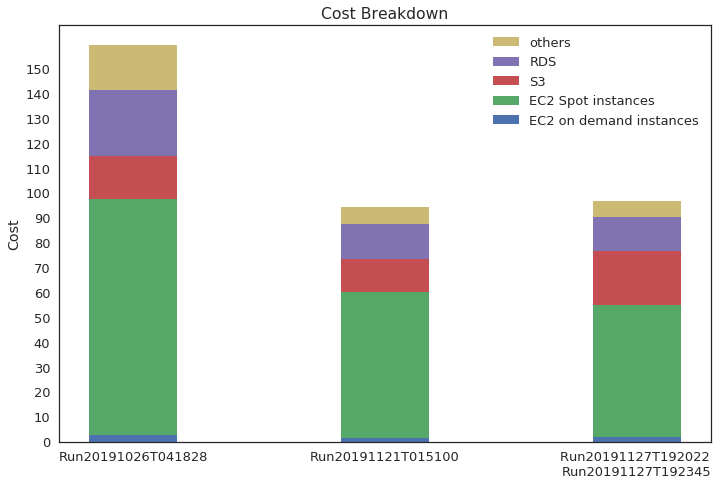
\includegraphics[width=0.7\textwidth]{billBreakdown.png}
\caption{Cost breakdown for each run}
\end{figure}



\section{Potential Improvements and more lessons learned} \label{future}

In this session we describe issues we have encountered during the execution and ideas to improve.
We discuss both intermittent failures that we understand and expect to occasionally encounter even in production, as well as higher level design or tooling improvements.

Failures can occur due to non-pipeline issues such as underlying infrastructure.
The fault rate may be small but as we scale up we start to encounter some.
Some examples are listed below; most seem transient.


\begin{enumerate}
\item Database connection timeout. Attempting to connect to the RDS instance failed.
\begin{lstlisting}[breaklines=true]
sqlalchemy.exc.OperationalError: (psycopg2.OperationalError) could not connect to server: Connection timed out
\end{lstlisting}
\item
After a file was added to a S3 bucket and during ingestion in the Butler registry, S3 reported a file does not exist.
This will be fixed in \jira{DM-22201}.
\begin{lstlisting}[breaklines=true]
FileNotFoundError: File at 's3://hsc-rc2-test1-hfc/repo-w38/hfc30/srcMatchFull/1316/srcMatchFull_1316_24_HSC_17.fits' does not exist; note that paths to ingest are assumed to be relative to self.root unless they are absolute.
\end{lstlisting}
\item S3 read timeout before science processing started in a job.
\begin{lstlisting}[breaklines=true]
botocore.exceptions.ReadTimeoutError: Read timeout on endpoint URL: "None"
\end{lstlisting}
\item Out-of-memory while running jobs.
For the same pipeline and input data, this is reproducible.
But we may not always have accurate memory usage prediction for any input data before running the jobs.
We can configure HTCondor to increase the memory requirement in the retry.
However sometimes OOM crashed the instances and appeared as a network issue, an undesirable behaviour.
\item Launching HTCondor Annex workers failed with connectivity check collector issues.
\begin{lstlisting}[breaklines=true]
Connectivity check found wrong collector (f5fc15573ffb9c93 vs a006066e73c412da).
\end{lstlisting}
\item Dataset ConflictingDefinitionError.
In rare occassions we observed dataset conflict errors from the registry without obvious reasons such as duplicate collection names or retries.
\jira{DM-21201} has refactored the code to robustify such transactions.
It could also be related to Spot instances getting terminated;
see next section on failure recovery.
\end{enumerate}


More generally, improvements in system design and tooling rise to prominence.
We discuss some ideas below.

\begin{enumerate}
\item Better job failure recovery strategies.
Our jobs write directly to the S3 bucket and the RDS instance via the Data Butler.
If a job fails in a state that partial outputs are written but the job does not fully finish, recovery is not trivial.
We may want a wrapper around the Pipeline Task that commits a transaction only if the job succeeds, have a reliable way to overwrite files from a failed job, or other ways to handle such scenarios.
\item Container based software stack.
We have found it tricky to handle the LSST stack installation, dependencies, and environments to be used together with other software.
One possible way to avoid the headaches is to use docker based stack releases.
This may also ensure consistency of software on the master and the workers more easily.
\item Better cluster management tooling.
Our current operational approach requires manually deploy suitable types and sizes of fleets based on our understanding of the overall workload.
Strategies on the instance choices and timing of requests therefore affect the cost, and manual adjustments are usually needed to reduce cost.
Annex can remove idle instances out of the condor pool but may not terminate the instances until the lease expires.
Also once instances drop out of the pool they can't be added back easily.
Tooling become essential for the operations.
For example we may use scripts to auto-scale the Annex condor pool.
An alternative approach is to use AWS Batch which automatically provisions the compute resources based on the workload and only charges for the actual resources used.
\item End-to-end CI.
This should include all operational components to do an end-to-end run.
This includes Butler repo generation, registry generation, Quantum Graph generation, job composition, workflow translation, job execution, and so on.
Many of the components were in the development phase and workarounds were used during the PoC.
For example a native Gen3 ingestion was not available so a Gen2-to-Gen3 conversion was needed.
As we put together the pieces, the absence of to do so in an automatic fashion became a key burden.
In retrospect we probably should have invested more time to automate the end-to-end workflow, even with workarounds.
Looking ahead a first step could be a \texttt{ci\_hsc} like package with the S3 backend.
\item Credential handling.
In this PoC the worker image carry credentials in files \texttt{~/.lsst/db-auth.yaml} and \texttt{~/.aws/credentials} which is not the best practice of handling the access.
\item Robustify and give better error messages.
It has been observed that sometimes the error messages could be misleading.

\end{enumerate}
